\chapter{Estrategia de modelos en entornos virtualizados}

Con el fin de abordar de manera ordenada la complejidad del sistema y validar progresivamente cada uno de sus componentes, se adoptó una estrategia basada en la construcción de modelos incrementales. Estos modelos permiten simular, probar y verificar distintas funcionalidades antes de integrarlas en la solución final.

Los modelos descritos a continuación tienen como finalidad:
\begin{itemize}
    \item Ligar problemas concretos a cada modelo y resolverlos de forma independiente. % Tener que debuggear todos en un solo modelo puede ser muy complejo.
    \item Obtener una solución funcional en un entorno virtualizado como último paso previo a implementarla sobre \textit{hardware}.
\end{itemize}

El detalle de cada modelo tiene como objetivo proporcionar una visión clara de su propósito, las validaciones que se intentan realizar y los aspectos que quedan fuera del alcance de cada uno. Además, en cada modelo se describen aspectos relevantes sobre las tecnologías utilizadas.

\section{Comunicando sitios seguros con WireGuard}
% Descripción del modelo
El primer modelo propuesto se centra en la comunicación entre múltiples sitios seguros a través de un túnel VPN configurado mediante WireGuard, permitiendo el acceso de los sitios a otros servicios en Internet por fuera del túnel. Se trata de un modelo de baja complejidad cuyo objetivo principal es familiarizarse con WireGuard y su configuración, así como utilizar herramientas como Wireshark para el análisis de paquetes de red. En una primera instancia, se implementó la topología de la figura \ref{diag:wg_minimal} utilizando GNS3, herramienta que permite instanciar y conectar múltiples máquinas virtuales, integrando herramientas de análisis de redes como Wireshark. 

Este modelo no pretende validar la arquitectura lógica del encriptador, sino que se enfoca en la configuración de WireGuard. Es por esto que cada encriptador se representa mediante una sola VM, en la cual se configura WireGuard. Se busca verificar que cada sitio pueda comunicarse con los demás a través del túnel VPN y acceder a Internet de manera directa.

Este modelo permite identificar y resolver problemas básicos de configuración de WireGuard, comprender el funcionamiento de las claves públicas y privadas, y analizar el tráfico cifrado y no cifrado mediante capturas en Wireshark.

\begin{figure}[h!]
    \centering
    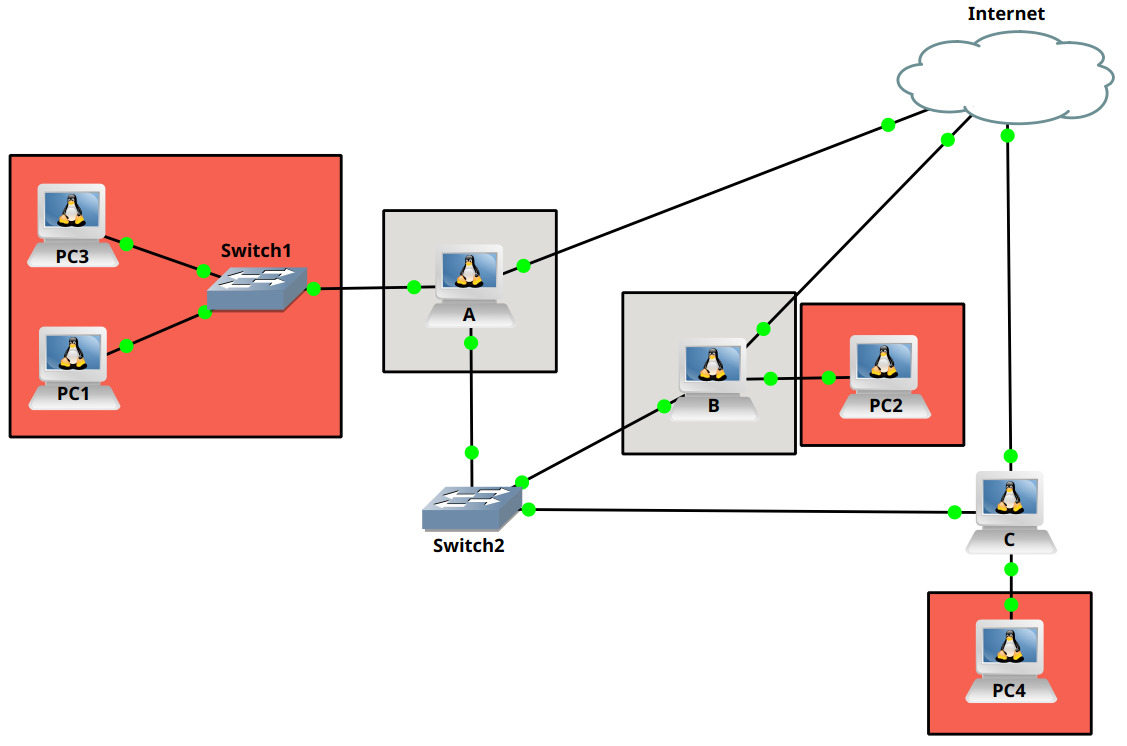
\includegraphics[width=0.6\textwidth]{../figs/gns3_1.png}
    \caption{Otro esquema mejorcito.}
    \label{diag:wg_minimal}
\end{figure}

En una siguiente iteración de este modelo se descartó la utilización de GNS3 y se optó por instanciar cada VM mediante QEMU% cosa que GNS3 ya lo hace en backend...
, adquiriendo mayor control sobre los dispositivos de red emulados. Un ejemplo de esto es la posibilidad de observar los parámetros PCI de las interfaces de red, lo cual es relevante para la implementación del \textit{passthrough} de las mismas en la solución final.

En este modelo, además, se valida el correcto funcionamiento tanto del kernel de Linux como del \textit{filesystem} inicial, modificados para incluir soporte para WireGuard. Estas imágenes serán posteriormente utilizadas en cada VMM gestionada por seL4.

\section{Introduciendo la arquitectura lógica del encriptador}
Una vez planteada la arquitectura lógica del sistema, se procedió con su simulación en GNS3. Este modelo permite limitar la complejidad de implementar la arquitectura a configurar la interconexión de las VMs que conforman el encriptador. Se tiene como objetivo validar la arquitectura lógica propuesta y verificar las funcionalidades de red pretendidas para el encriptador como lo es el \textit{split-tunneling}.

En la figura \ref{diag:gns3_2} se muestra la topología del modelo en GNS3 para simular el sistema completo. Aquí el encriptador se implementa como una interconexión mediante interfaces de red de tres VMs independientes. 

\begin{figure}[h!]
    \centering
    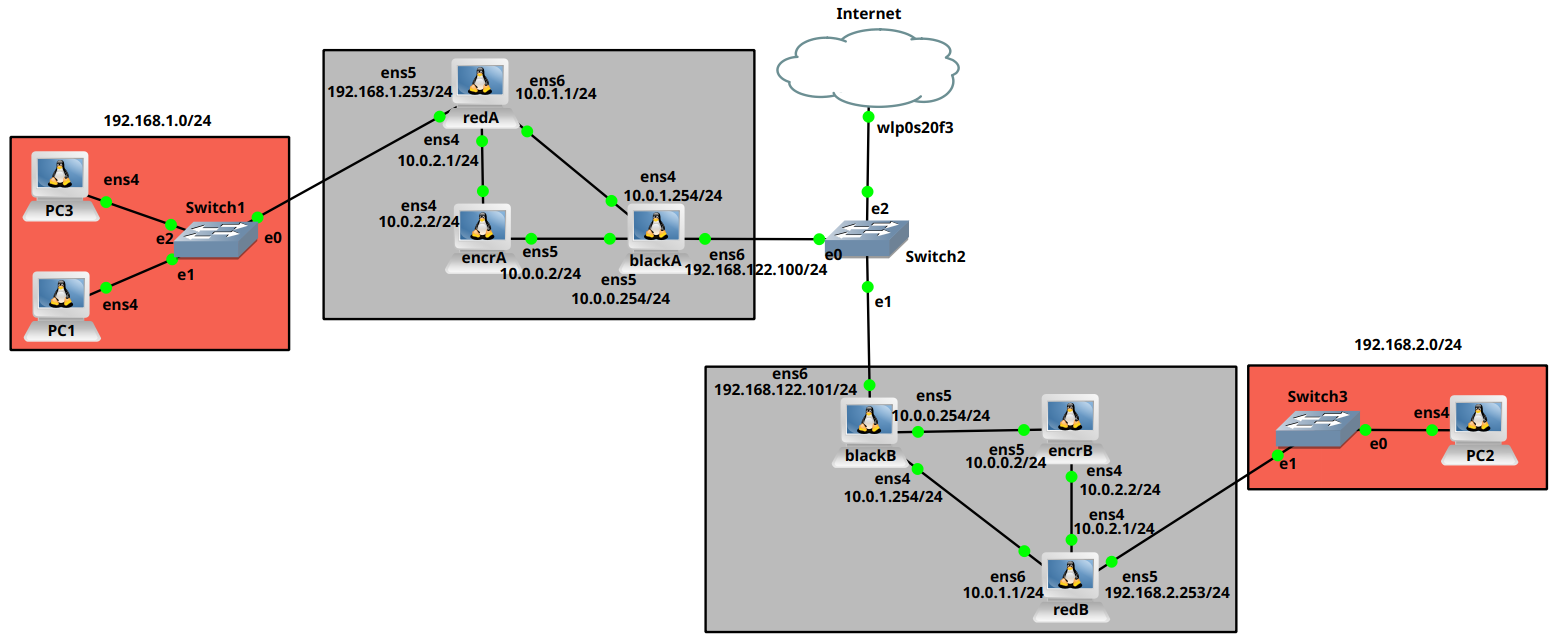
\includegraphics[width=0.8\textwidth]{../figs/gns3_2.png}
    \caption{Otro esquema mejorcito.}
    \label{diag:gns3_2}
\end{figure}

Como \textit{output} de este modelo se obtienen las configuraciones de red necesarias, como tablas de enrutamiento y reglas de firewall, para darle al encriptador la funcionalidad pretendida. Estas configuraciones se utilizarán posteriormente en la solución.

\section{Utilizando seL4 como hipervisor}
El siguiente modelo se centra en la lograr la comunicación entre dos VM, las cuales se encuentran en instancias independientes de seL4 funcionando como hipervisor. Este modelo tiene como objetivo validar el \textit{passthrough} de hardware, en este caso, de una interfaz de red entre seL4 y el \textit{guest} Linux. En la figura \ref{diag:esquema_passthrough} se esquematiza la topología del modelo.

\begin{figure}[h!]
    \centering
    \includegraphics[width=0.5\textwidth]{example-image}
    \caption{Dos VMs con un passthrough, ping 2VM.}
    \label{diag:esquema_passthrough}
\end{figure}

Un paso importante de este desarrollo es validar la compatibilidad de las imágenes de Linux obtenidas previamente con el hipervisor seL4. Para ello, en este modelo se utiliza el \textit{output} del primer modelo, la imagen de Linux con soporte para WireGuard.

Como \textit{output} de este modelo se tiene la configuración adecuada para realizar el \textit{passthrough} de un dispositivo de red al Linux \textit{guest}. Además de correcciones que se hayan hecho sobre la imagen de Linux para lograr la compatibilidad con el VMM de seL4.

\section{Implementando el encriptador en seL4}
Este modelo se centra en integrar los desarrollos realizados en los modelos anteriores, y obtener así una solución completa como paso previo a su despliegue sobre \textit{hardware} real. Aquí se validan en conjunto todas las funcionalidades y configuraciones obtenidas previamente, asegurando la interoperabilidad de los distintos componentes en un entorno virtualizado.

Este modelo utiliza uno de los ejemplos de uso de VMs en CAmkES, el proyecto \textit{zmq\_samples}, como base para la implementación del encriptador. Este ejemplo permite la comunicación entre dos VMs utilizando ZeroMQ, una biblioteca de mensajería asíncrona que facilita la comunicación entre procesos a través de regiones de memoria compartida definidas. Cada VM contiene una interfaz de red virtual \textit{eth0} que se conecta a las interfaces \textit{eth0} de las demás. En la figura \ref{diag:model4} se esquematiza el sistema completo.

\begin{figure}[h!]
    \centering
    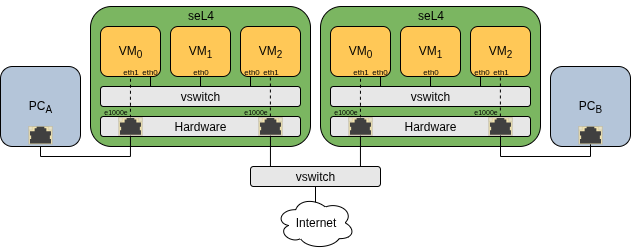
\includegraphics[width=0.8\textwidth]{../figs/3_model4.png}
    \caption{Esquema del encriptador con seL4 simulado en QEMU.}
    \label{diag:model4}
\end{figure}

\pdfcomment{
Describir el cambio de topología respecto a la figura \ref{diag:gns3_2}. ¿Por qué esto no afecta?}

